% Years before a place fills its first block, t = ln 2 / ln(1 + r), Eq. (8).
\documentclass[border=2mm]{standalone}
\usepackage{fontspec}\setmainfont{LibertinusSans}[Extension=.otf,UprightFont=*-Regular,BoldFont=*-Bold]
\usepackage{unicode-math}\setmathfont{LibertinusMath-Regular.otf}
\usepackage{pgfplots}\pgfplotsset{compat=1.18}
\providecommand{\T}[2]{#1}% \T{English}{French}; the -fr wrappers select the French text
\pgfkeys{/pgf/number format/.cd, 1000 sep={\,}}\ifdefined\figfr\pgfkeys{/pgf/number format/use comma}\fi
\begin{document}
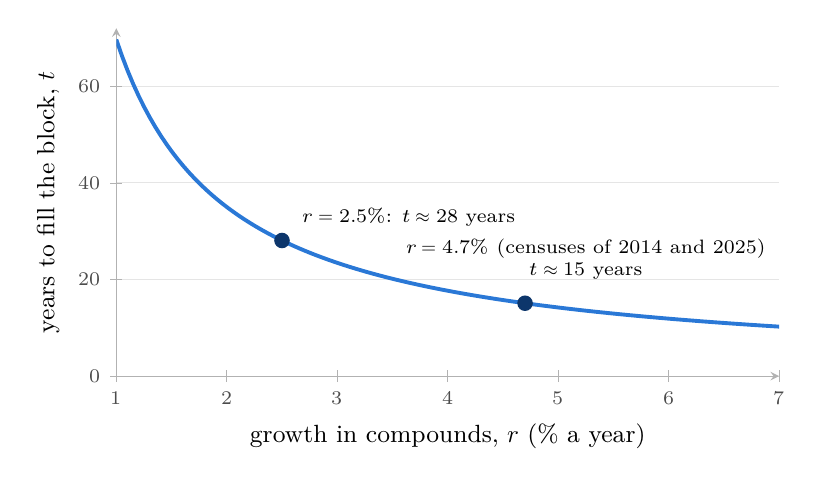
\begin{tikzpicture}
\begin{axis}[width=10cm, height=6cm, xmin=1, xmax=7, ymin=0, ymax=72,
  axis lines=left, axis line style={gray!60}, tick style={gray!60}, tick label style={font=\scriptsize, text=black!70},
  xlabel={\T{growth in compounds, $r$ (\% a year)}{croissance des concessions, $r$ (\% par an)}}, ylabel={\T{years to fill the block, $t$}{années avant de remplir le bloc, $t$}}, label style={font=\small},
  ymajorgrids, grid style={gray!20}]
\addplot[domain=1:7, samples=120, line width=1.4pt, color={rgb,255:red,42;green,120;blue,214}] {ln(2)/ln(1+x/100)};
\addplot[only marks, mark=*, mark size=2.6pt, color={rgb,255:red,13;green,54;blue,107}] coordinates {(2.5,28.07) (4.7,15.09)};
\node[anchor=south west, font=\scriptsize] at (axis cs:2.6,29) {\T{$r=2.5\%$: $t\approx28$ years}{$r=2{,}5\%$ : $t\approx28$ ans}};
\node[anchor=south, font=\scriptsize, align=center] at (axis cs:5.25,18) {\T{$r=4.7\%$ (censuses of 2014 and 2025)\\$t\approx15$ years}{$r=4{,}7\%$ (recensements de 2014 et 2025)\\$t\approx15$ ans}};
\end{axis}
\end{tikzpicture}
\end{document}
